% PlanArena paper. Numbers and tables are filled from results/ by planarena/paper.py: edit this template, then run
%   python -I -m planarena.paper      (writes paper.tex and, with tectonic, paper.pdf). Do not edit paper.tex.
% Citations are numbered; for an author-year journal use [authoryear,round] and plainnat below.
\documentclass[10pt]{article}
\usepackage[margin=0.8in]{geometry}
\usepackage{fontspec}
\setmainfont{texgyretermes}[Extension=.otf, UprightFont=*-regular, BoldFont=*-bold,
  ItalicFont=*-italic, BoldItalicFont=*-bolditalic]
\usepackage{microtype}
\usepackage{booktabs}
\usepackage{graphicx}
\usepackage{amsmath}
\usepackage{placeins}
\usepackage[numbers,sort&compress]{natbib}
\usepackage[hidelinks]{hyperref}
\usepackage{tikz}
\usetikzlibrary{arrows.meta,positioning,calc}
\usepackage{caption}
\captionsetup{font=footnotesize,labelfont=bf,skip=3pt}
\usepackage{enumitem}
\setlist{nosep,leftmargin=*}
\usepackage[compact]{titlesec}
\titlespacing*{\section}{0pt}{8pt}{3pt}
\titlespacing*{\subsection}{0pt}{6pt}{2pt}
\titlespacing*{\paragraph}{0pt}{3pt}{0.6em}
\setlength{\parskip}{0.15em}
\setlength{\emergencystretch}{1.5em}
\setlength{\textfloatsep}{8pt plus 2pt minus 2pt}
\setlength{\floatsep}{6pt plus 2pt minus 2pt}
\setlength{\intextsep}{6pt plus 2pt minus 2pt}
\setlength{\bibsep}{1pt}
\renewcommand{\bibfont}{\footnotesize}
\graphicspath{{../docs/figures/}}

\title{\vspace{-2em}\large\textbf{PlanArena: an integrated land-use optimizer with empirical evaluation}\\[0.2em]
\normalsize Measuring the multidimensional impact of land-use decisions, with stakeholder interests as votes,\\
on official data for ten US cities}
\author{\normalsize Anonymous author (withheld for double-blind review)}
\date{\footnotesize Draft, \today}

\begin{document}
\maketitle
\vspace{-1.5em}

\begin{abstract}
\noindent Deciding which land uses go where is a location-allocation problem with multidimensional effects: a change
alters homes, jobs, access to services, the tax base, emissions and runoff, interacts with neighbouring parcels, and
may never be built. US cities decide such changes at public hearings, where residents testify but do not vote.
PlanArena is an open land-use optimizer that measures these effects and represents stakeholder interests as votes. It
scores any parcel-level change on 11 indicators with sensitivity ranges in 46 ms
(Manhattan) to 0.58 s (New York City), estimates how likely a change is, recommends plans within zoning and
precedent, and compares nine voting rules over simulated stakeholders, on official data for 4{,}995{,}208 parcels
in ten US cities. On held-out Manhattan lots, given what was built, predicted changes correlated with recorded homes
($r = 0.79$) and emissions ($r = 0.60$), above a gradient-boosted baseline, but overstated total homes
1.47-fold and had no skill for jobs. Redevelopment was ranked out of time with AUC
0.851--0.902, but observed-to-predicted event ratios ranged 0.07--1.70 across years.
Likelihood weighting brought housing projections from 76--193 to 0.80--2.60 times what was
built; a five-year trend ranked districts better than build-out projections. Searches were checked against exhaustive enumeration; the
votes are illustrative.

\smallskip\noindent\textbf{Keywords:} land-use optimization; location allocation; impact assessment; planning support
systems; computational social choice; model validation
\end{abstract}

\section{Introduction}

Deciding which land uses go where (housing, jobs, services, open space) is a location-allocation problem
\citep{church1974,revelle2005}. Its effects are hard to measure for four reasons.
\begin{itemize}
\item \textbf{Many dimensions.} One change alters homes, jobs, access to shops, parks and facilities, the tax base,
energy use and runoff, and these trade off against each other \citep{malczewski2006,rahman2021}.
\item \textbf{Spatial interaction.} Effects spread to neighbouring parcels through walking distance, land-use mix and
competition for development \citep{verburg2004}.
\item \textbf{Uncertainty.} A permitted change may never be built. In three Manhattan rezonings replayed here,
capacity projected 8{,}423 homes on development sites; 561 were built by 2025.
\item \textbf{Competing interests.} Residents, developers, businesses, environmental advocates and city finances weigh
these effects differently, and no single answer is correct \citep{rittel1973}.
\end{itemize}

\paragraph{How decisions are made today.} In US cities, rezonings and plan amendments are decided at public hearings.
\begin{itemize}
\item \textbf{The process.} Planning staff prepare a report, and large rezonings, such as those replayed here, add an
environmental review that projects development on identified sites. Residents and advocates testify; the planning
commission and the council vote.
\item \textbf{Testimony is advisory.} Residents are heard but do not vote. Speakers at planning and zoning meetings are
disproportionately older, male, long-time homeowners \citep{einstein2019}, and legally required hearings meet few
goals of participation \citep{arnstein1969,innes2004,fung2006}.
\item \textbf{Fragmented evidence.} Environmental, fiscal and access effects arrive as separate studies, if at all, and
are rarely weighed together.
\end{itemize}

\paragraph{What computation can measure.} Each part of the problem now has a technical tool:
\begin{itemize}
\item \textbf{parcel-level impact models} calibrated on observed records, which measure many indicators at once;
\item \textbf{supervised learning on parcel histories}, tested out of time, which estimates how likely a change is
\citep{tepe2020,carruthers2024};
\item \textbf{graph neural networks} over parcel adjacency, which represent spatial dependence;
\item \textbf{many-objective evolutionary search} \citep{deb2014}, which explores the combinatorial space of plans;
\item \textbf{computational social choice and bargaining} \citep{nash1950,brandt2016}, which turn stakeholder
preferences into a decision. Game-theoretic simulation has been applied to collective land-use decisions
\citep{abolhasani2022}.
\end{itemize}
Planning support systems (PSS) and urban digital twins aim to combine such tools
\citep{klosterman1999,geertman2020,batty2018,lehtola2022}. Three gaps remain:
\begin{itemize}
\item \textbf{Untested outputs.} Their outputs are seldom tested against outcomes \citep{vonk2005,lei2023,azadi2025,
kruse2026}.
\item \textbf{Optimization.} It rarely asks whether recommended changes are plausible, or how the choice depends on the
decision rule \citep{zheng2023,feng2024,lin2025}.
\item \textbf{Fragmented data.} The data are spread across agencies and schemas, some only as documents:
Philadelphia's land-use plan exists only as maps in 17 PDF district plans.
\end{itemize}

\paragraph{This paper.} PlanArena is an open land-use optimizer that measures the impact of any parcel-level change
and makes stakeholder interests part of the decision. It contributes:
\begin{enumerate}
\item \textbf{Measurement.} Any edit is scored on 11 indicators in three pillars, with sensitivity
ranges, at interactive speed. Each edit also shows what exists, what zoning permits, what the plan intends and how
likely the change is.
\item \textbf{Optimization and decision.} The optimizer recommends plans within zoning and precedent. Resident,
environmental, business, developer and fiscal interests vote on candidate plans under nine rules, and residents also
vote block by block.
\item \textbf{Official data for ten cities.} Existing use, plan and zoning for 4{,}995{,}208 parcels are on one
schema, with a validated method to digitise plans published as vector PDF maps.
\item \textbf{Empirical evaluation where data allow} (Table~\ref{tab:design}): held-out and out-of-time tests of
impacts, likelihood and projections, exhaustive checks of the searches, and the type of evidence behind each claim,
with design guidance drawn from the results.
\end{enumerate}
\textbf{Scope.} Impacts are evaluated in Manhattan only; elsewhere coefficients are national or regional. Zoning is
represented by use permissions and maximum floor-area ratios, access by straight-line distance. Votes rest on assumed
utilities, not elicited preferences, and usability with planners is not evaluated. A technical supplement specifies
every model and test.

\section{Related work}\label{sec:related}

\paragraph{PSS and urban digital twins.} PSS combine suitability, demand projection and allocation for scenario
planning \citep{klosterman1999,geertman2020}, often in a geodesign workflow linking representation, change, impact
and decision \citep{steinitz2012}. Their limited use and uncertain usefulness are long-standing concerns
\citep{vonk2005,tebrommelstroet2013,pelzer2017}. Digital twins extend them to integrated, updatable city models
\citep{batty2018,batty2024,white2021,lehtola2022,ferrebigorra2022}. Reviews report technical and organisational
barriers \citep{lei2023,wu2025}, and ambitions ahead of demonstrated contributions \citep{azadi2025,luo2025,kruse2026}.
PlanArena attaches a test against observed data to each output.

\paragraph{Optimization and collective decisions.} Location-allocation models site facilities and uses
\citep{church1974,revelle2005}; multicriteria analysis and multi-objective optimization generate and rank land-use
alternatives \citep{malczewski2006,rahman2021}. Recent work uses deep reinforcement learning
\citep{zheng2023} and explicit stakeholder interests \citep{feng2024,lin2025}. Planning problems have no single correct
solution \citep{rittel1973}, so the rule that turns preferences into a choice matters. Bargaining \citep{nash1950} and
voting rules \citep{schulze2011,brandt2016} have different properties, and bargaining has been combined with land
reallocation \citep{hashemi2026}. Simulated votes are not participation \citep{arnstein1969}; PlanArena uses them
only to show how a choice depends on its rule.

\paragraph{Predicting development, and regulation.} Urban change models range from cellular automata
\citep{clarke1997} and statistical site models \citep{landis1998} to behavioural \citep{waddell2002,waddell2003} and
agent-based simulation \citep{parker2003}, with neighbourhood and temporal effects as priorities
\citep{verburg2004,weerasinghe2025}.
\begin{itemize}
\item \textbf{Parcel models} capture existing and historical neighbourhood conditions \citep{tepe2020}, and machine
learning complements econometrics \citep{carruthers2024}.
\item \textbf{Redevelopment} depends on land value relative to the structure \citep{rosenthal1994,dye2007}. In
Chicago, smaller and older buildings with less lot coverage are replaced more often \citep{weber2006,charles2013}.
\item \textbf{Regulation is not exogenous.} Rezoning follows development opportunity \citep{gabbe2018}, studies differ
on upzoning's short-run effect on construction \citep{freemark2020,dong2024,greenaway2023}, and plans are only partly
implemented \citep{talen1996,laurian2004,brody2005,berke2006,loh2011}.
\item \textbf{Regulation in models.} Recent land-change models integrate zoning and planning rules
\citep{hersperger2018,domingo2021,abolhasani2026} but do not test what they add to prediction on held-out history.
\end{itemize}

\paragraph{Validation.} Land-change predictions should be compared with persistence at several resolutions
\citep{pontius2008,pontius2011}, and their transition probabilities validated directly \citep{black2023}. Under
spatial and temporal dependence, random cross-validation overstates skill \citep{roberts2017,ploton2020}, and models
apply only where new data resemble the training data \citep{meyer2021}. Uncertainty from many coefficients is better
assessed by varying them jointly \citep{saltelli2019}.

\section{The system}\label{sec:system}

A parcel twin holds each city's official layers (Figure~\ref{fig:arch}). Four engines answer the planner's questions:
\begin{itemize}
\item the \textbf{impact engine}: what would a change do?
\item the \textbf{likelihood models}: is it likely?
\item the \textbf{optimizer}: what would do better?
\item the \textbf{decision module}: who would choose it, and under which rule?
\end{itemize}
In the Studio, a browser application, a planner paints uses and floor-area ratios on parcels and sees every
indicator, flag and recommendation update (Figure~\ref{fig:studio}).

\begin{figure}[t]
\centering
\resizebox{0.78\linewidth}{!}{%
\begin{tikzpicture}[every node/.style={font=\footnotesize, align=center},
  box/.style={draw, rounded corners=2pt, minimum height=9mm, text width=30mm, fill=gray!6},
  q/.style={font=\footnotesize\itshape, text width=30mm, align=left},
  arr/.style={-{Stealth[length=2mm]}}]
\node[box] (src) at (-2.2, 0) {Official layers and\\assessor records};
\node[box] (pdf) at (2.2, 0) {Plans published as\\PDF maps (digitised)};
\node[box, text width=44mm] (twin) at (0, -1.6) {Parcel twin: existing use, zoning\\and plan (official, ten cities)};
\node[box] (imp) at (-2.2, -3.3) {Impact engine\\11 indicators, ranges};
\node[box] (lik) at (2.2, -3.3) {Likelihood\\redevelopment, precedent};
\node[box, text width=44mm] (opt) at (0, -5.0) {Optimizer\\NSGA-III, exact re-scoring};
\node[box, text width=44mm] (dec) at (0, -6.6) {Decision module\\nine voting rules, bargaining};
\node[box, text width=60mm] (ui) at (0, -8.1) {Studio and game $\cdot$ exports $\cdot$ ArcGIS Urban};
\node[q, anchor=east] at (-4.2, -3.3) {What would it do?};
\node[q, anchor=west] at (4.2, -3.3) {Is it likely?};
\node[q, anchor=west] at (3.0, -5.0) {What would do better?};
\node[q, anchor=west] at (3.0, -6.6) {Under which rule?};
\draw[arr] (src) -- (twin); \draw[arr] (pdf) -- (twin);
\draw[arr] (twin) -- (imp); \draw[arr] (twin) -- (lik);
\draw[arr] (imp) -- (opt); \draw[arr] (lik) -- (opt);
\draw[arr] (opt) -- (dec); \draw[arr] (dec) -- (ui);
\end{tikzpicture}}
\caption{Architecture. Every number the system shows comes from one of these components, each tested on observed
data (Table~\ref{tab:design}).}
\label{fig:arch}
\end{figure}

\begin{figure}[t]
\centering
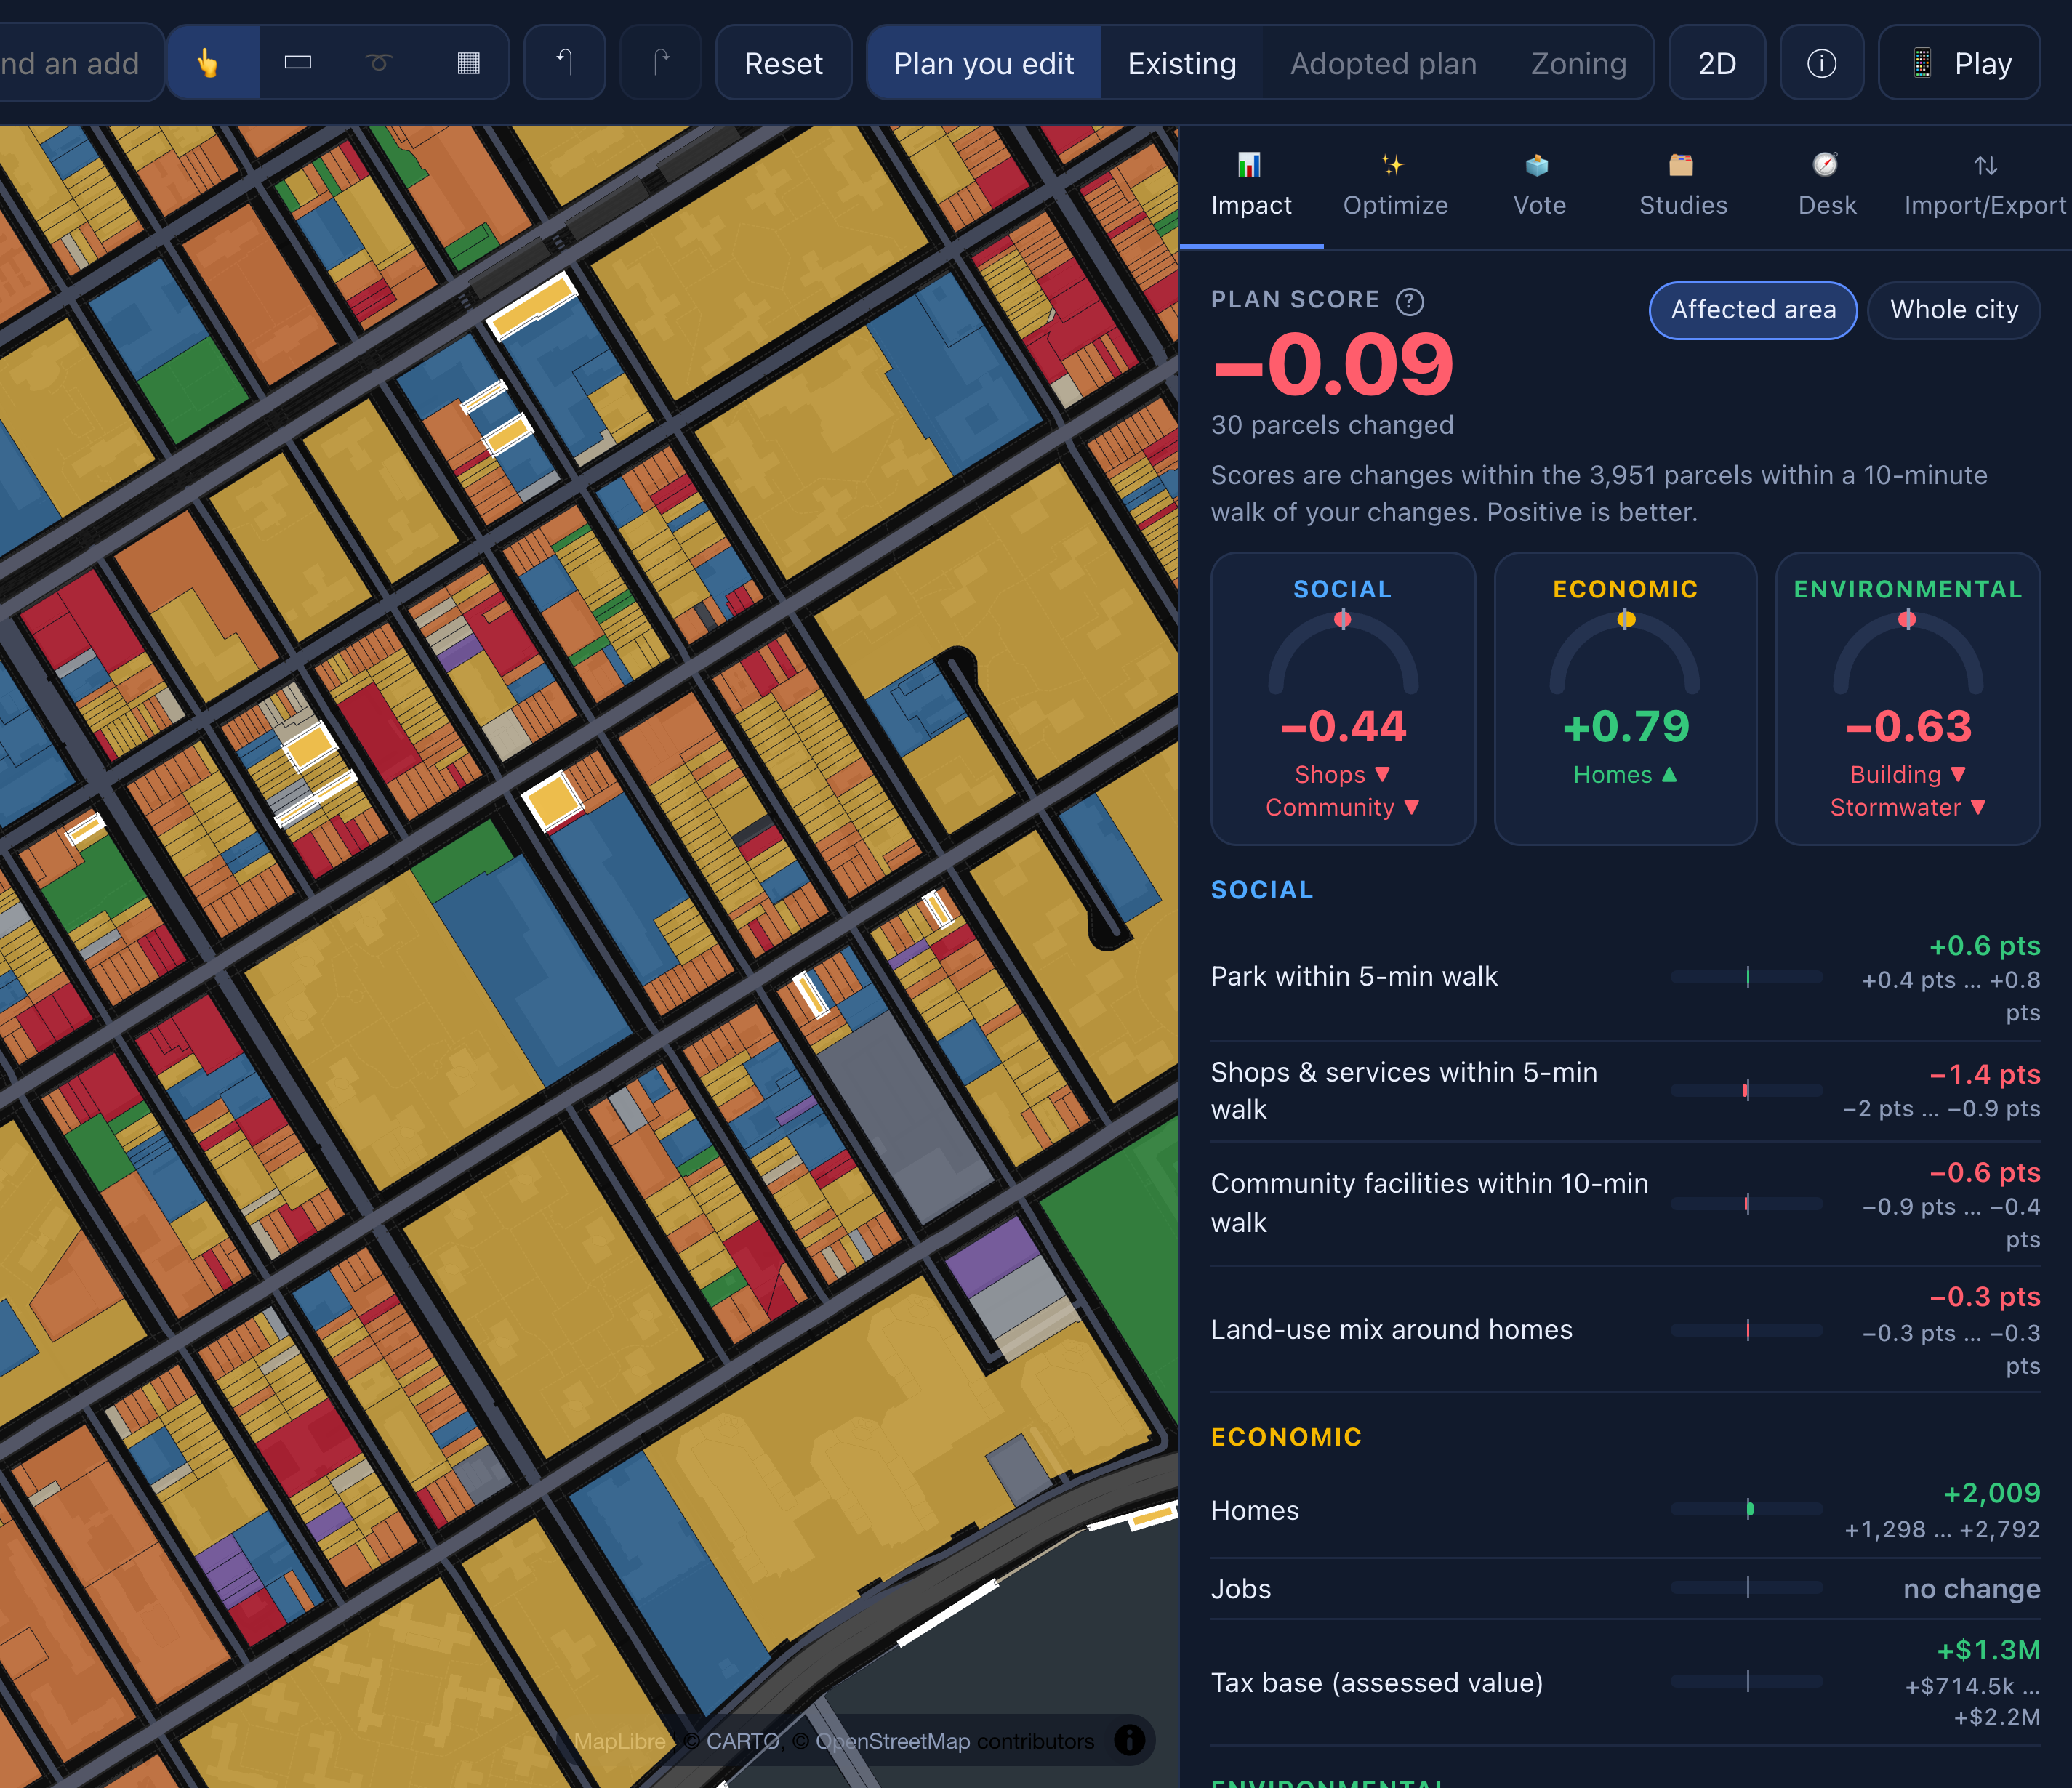
\includegraphics[width=0.85\linewidth]{ui_impact_crop.png}
\caption{The Studio in Manhattan: thirty parking lots and vacant parcels in East Harlem painted as housing
(outlined). Right: plan score, social, economic and environmental pillars, and each indicator's change within a
ten-minute walk with its sensitivity range. Top: switches between the plan being edited and the city's existing,
planned and zoned use. The use palette, left of the map, is not shown.}
\label{fig:studio}
\end{figure}

\paragraph{Parcel twin and official layers.} The twin covers the nine largest US cities except San Jose, plus
Milwaukee (Table~\ref{tab:cities}).
\begin{itemize}
\item \textbf{Existing land use} is the parcel land use the city or its regional planning agency publishes, refined
with assessor records where the layer groups uses.
\item \textbf{The adopted plan} (future land use) and \textbf{zoning} are separate layers.
\item \textbf{Classes.} Explicit crosswalks map every source code to 16 classes: three housing types, mixed use,
retail, office, hotel, industry, warehousing, education, health, civic, open space, transportation, parking and
vacant land. The classes nest in nine analysis groups.
\item \textbf{Records.} Floor area, homes, year built and assessed value come from assessor or city records, with
estimated fields flagged. Jobs are fitted to LEHD block counts.
\item \textbf{Provenance.} Inputs are downloaded by script, with URL and SHA-256 hash recorded.
\item \textbf{Philadelphia's plan}, published only as PDF maps, is digitised (Appendix~\ref{app:digitise}):
15 of 17 plans, covering 83\% of parcels, with median registration errors of
1.1--7.2 ft, each checked against a shifted-map control.
\item \textbf{Missing plans.} Where a city publishes no plan as data, the layer is absent, not estimated.
\end{itemize}

\begin{table}[t]
\centering
\scriptsize
\setlength{\tabcolsep}{4pt}
\caption{The ten cities: official parcel layers on one schema. Shares are of the city's parcels.}
\label{tab:cities}
\begin{tabular}{lrllllll}
\toprule
City & Parcels & Existing use (source) & Share & Adopted plan & Share & Zoning & Homes / Census \\
\midrule
New York & 856{,}634 & MapPLUTO (City Planning) & 100\% & none citywide & -- & 100\% & 1.03 \\
Los Angeles & 672{,}444 & SCAG 2020; county assessor & 100\% & General Plan (SCAG 2019) & 100\% & 100\% & 0.99 \\
Chicago & 606{,}894 & CMAP 2023; county assessor & 100\% & none citywide & -- & 96\% & 1.05 \\
Houston & 630{,}525 & City (appraisal codes) & 97\% & none & -- & -- & 0.95 \\
Phoenix & 510{,}871 & County assessor; MAG & 100\% & General Plan & 100\% & 99\% & 0.99 \\
Philadelphia & 547{,}410 & City Planning Commission; OPA & 100\% & district plans (digitised PDF) & 83\% & 100\% & 0.99 \\
San Antonio & 438{,}009 & Bexar Appraisal District & 100\% & adopted area plans & 61\% & 82\% & 0.99 \\
San Diego & 272{,}948 & SANDAG 2025; county assessor & 100\% & General and community plans & 100\% & 94\% & 1.02 \\
Dallas & 311{,}431 & City 2026; DCAD & 100\% & forwardDallas! 2.0 & 99\% & 79\% & 0.98 \\
Milwaukee & 148{,}042 & MPROP & 100\% & PDF only (not included) & -- & 99\% & 1.06 \\
\textit{All} & 4{,}995{,}208 &  &  &  &  &  &  \\
\bottomrule
\end{tabular}
\par\smallskip
\begin{minipage}{0.95\linewidth}\footnotesize Existing use is the city's or regional agency's parcel land use, refined by assessor records where the layer groups uses. Homes / Census: homes in the twin over Census 2020 housing units. Houston has no zoning. Milwaukee's area plans are published as PDFs that could not be downloaded by script.\end{minipage}
\end{table}

\paragraph{Impact engine.} An edit sets a parcel's use and, optionally, its floor-area ratio (FAR). The engine
computes the 11 indicators of Table~\ref{tab:indicators} within a ten-minute walk and citywide.
\begin{itemize}
\item \textbf{Unchanged parcels} keep their observed values, so the baseline reproduces the records exactly.
\item \textbf{Changed parcels} follow a hybrid delta rule. A density-only change on a consistent record scales the
observed composition; a use change removes the observed old use and adds the modelled new one (Supplement S3).
\item \textbf{Derived quantities.} Homes follow from residential floor area and the parcel's floor area per home.
Jobs follow from floor-area components and rates fitted to LEHD counts. Emissions follow from energy intensities and
emission factors derived from New York's benchmarking data (Local Law 84) and emission limits (Local Law 97).
Runoff follows from surface coefficients, and value from the difference between modelled values.
\item \textbf{Access, mix and green cover} are recomputed on a 50 m raster within straight-line radii of 400 m and
800 m, not along walking routes.
\item \textbf{Ranges.} Every coefficient has a source and a status, and low and high variants give each indicator a
sensitivity range. A range has no probability attached and is not a prediction interval.
\end{itemize}
Indicator scores are per cent changes (totals) or percentage points (shares) against the scope's baseline, clipped to
$\pm 100$; a pillar is the mean of its indicators, and the overall score a weighted mean of pillars with weights the
planner sets. Scoring a 50-parcel edit, ranges included, takes
46 ms on Manhattan's 42{,}075 parcels and 0.58 s on New York City's 856{,}634.
Impacts are computed for the nine analysis groups, for which the coefficients are calibrated and validated.

\begin{table}[t]
\centering
\scriptsize
\setlength{\tabcolsep}{4pt}
\caption{Indicators computed for every edit, and how each is tested (Manhattan).}
\label{tab:indicators}
\begin{tabular}{lllll}
\toprule
Indicator & Pillar & Unit & Better & Test \\
\midrule
Homes & economic & units & higher & held-out change \\
Jobs & economic & jobs & higher & existing; change: no skill \\
Tax base (assessed value) & economic & USD & higher & held-out change \\
Park within 5-min walk & social & \% of residents & higher & not validated \\
Shops \& services within 5-min walk & social & adequacy 0-1 & higher & not validated \\
Community facilities within 10-min walk & social & adequacy 0-1 & higher & not validated \\
Land-use mix around homes & social & index 0-1 & higher & not validated \\
Green \& open space & environmental & acres & higher & direct accounting \\
Stormwater runoff & environmental & impervious-equiv. acres & lower & not validated \\
Building emissions & environmental & tCO2e / yr & lower & existing; held-out change \\
Green cover near homes & environmental & \% of land within 400 m & higher & not validated \\
\bottomrule
\end{tabular}
\par\smallskip
\begin{minipage}{0.95\linewidth}\footnotesize Unchanged parcels keep their observed values; changed parcels follow the delta equations. Each indicator carries a sensitivity range from low and high coefficient variants. Access, mix, green cover and runoff are recomputed from the resulting state but have no observed after-change data to test against.\end{minipage}
\end{table}

\paragraph{Likelihood, precedent and pattern.} Three models judge plausibility.
\begin{itemize}
\item \textbf{Redevelopment.} A gradient-boosted model (LightGBM), trained only on outcomes known at the decision
year, gives each lot's probability of redevelopment within one, three or five years and its likely new use. Its
inputs are the lot's use, size, built and permitted floor area, age and land share of value, its neighbourhood and its
zoning.
\item \textbf{Precedent.} A conversion is flagged if buildings of that use and size were not converted to the proposed
use in the past decade.
\item \textbf{Pattern.} A graph neural network over parcel adjacency, combined with LightGBM, describes how well a use
fits its surroundings: an existing pattern, not a norm.
\end{itemize}
Edits that depart from the plan or from what zoning allows are flagged (Figure~\ref{fig:inspector}).

\begin{figure}[t]
\centering
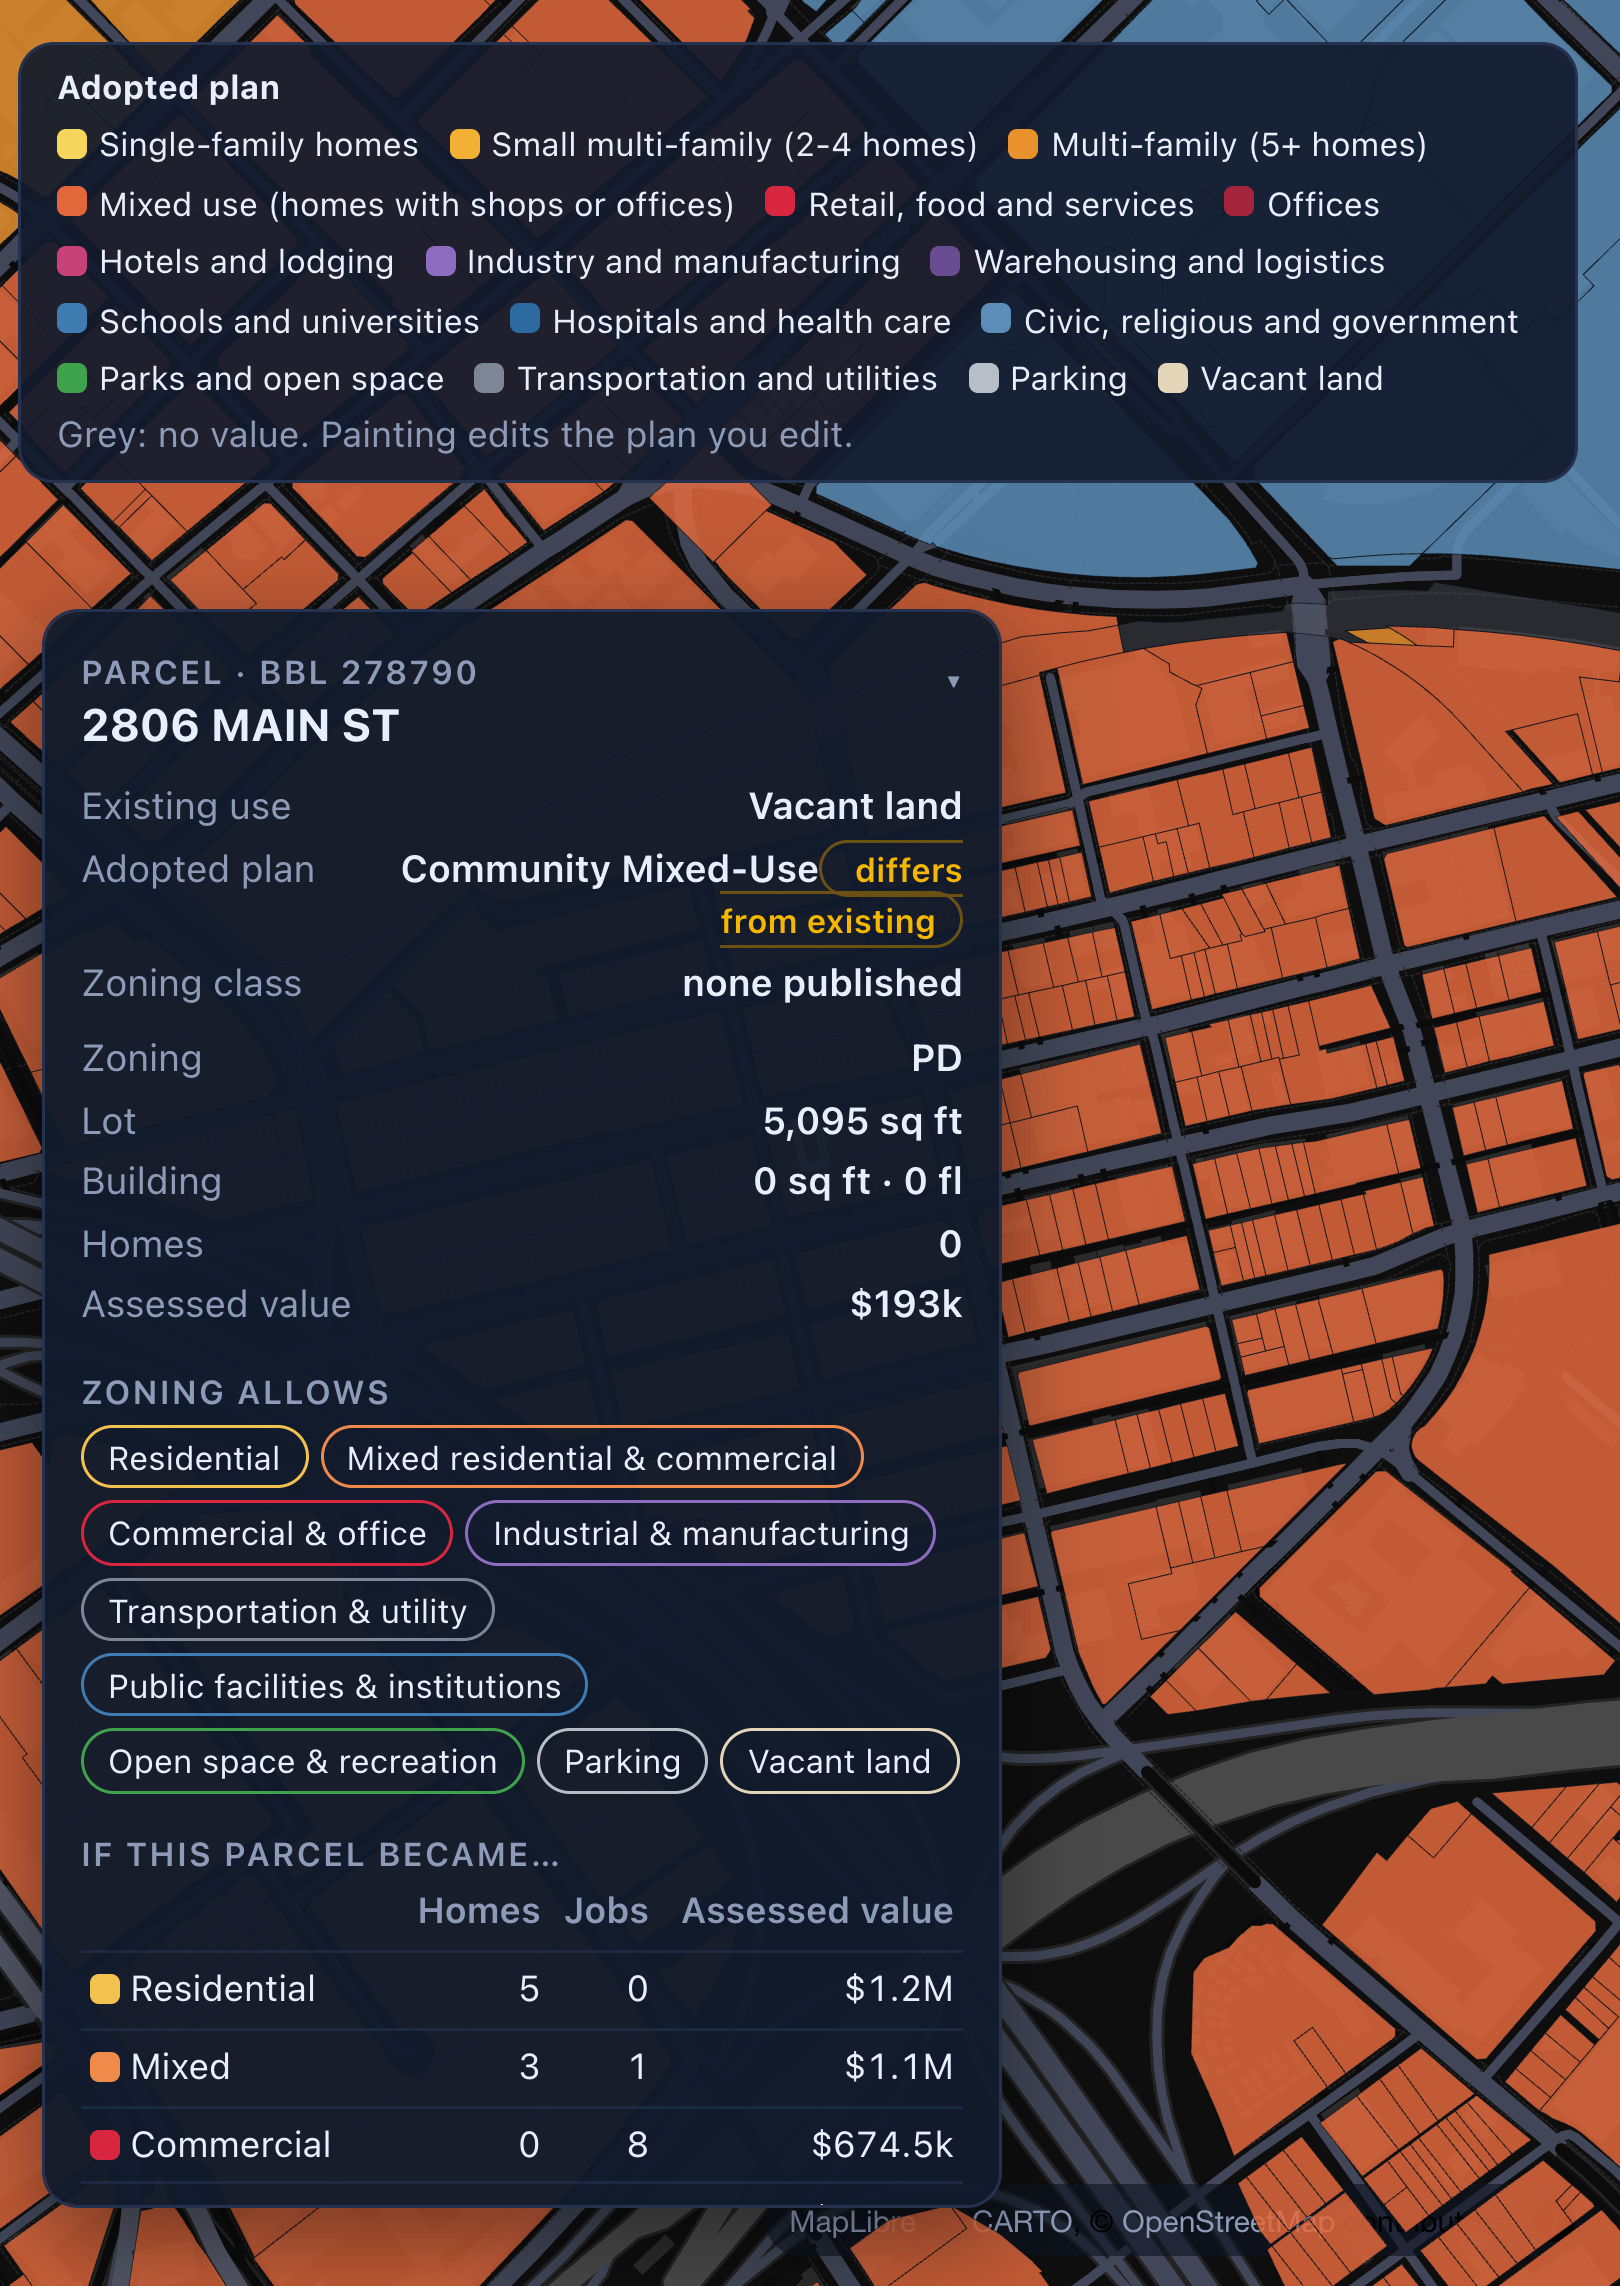
\includegraphics[width=0.5\linewidth]{ui_inspector.png}
\caption{Parcel inspector on the adopted-plan layer (Dallas). For a vacant lot the plan designates Community
Mixed-Use, it lists existing use, plan designation (flagged as differing), zoning, the uses zoning allows, and what each
new use would yield in homes, jobs and assessed value.}
\label{fig:inspector}
\end{figure}

\paragraph{Optimizer.} The optimizer maximizes the overall score minus a penalty per conversion, under a budget of
changes. The uses zoning permits are a hard constraint, existing homes and protected sites are kept, conversions
without precedent are skipped, and candidates can be restricted to the parcels most likely to be redeveloped. Two
searches are offered:
\begin{itemize}
\item iterated best response over first-order move estimates, with exact re-scoring of the best moves;
\item NSGA-III \citep{deb2014}, which returns a Pareto set across the three pillars, re-scored exactly.
\end{itemize}
Both report the best plan found, not a proven optimum (Supplement S6).

\paragraph{Decision module.} Choices are contested \citep{rittel1973}, so the module shows how the chosen plan depends
on the decision rule.
\begin{itemize}
\item \textbf{Agents.} Five stakeholder agents (residents, business, developers, environmental and city-finance
interests) score candidates from assumed utilities over the indicators.
\item \textbf{Rules.} Nine voting rules are compared with the Nash bargaining solution \citep{nash1950} and a
residents' referendum by block. Schulze's method \citep{schulze2011} decides.
\item \textbf{Reports.} Whether a Condorcet winner exists, whether one insincere ballot could change the outcome, and
the winner's robustness to coefficients and seats.
\end{itemize}
Unlike hearing testimony, these interests are votes: each agent holds one seat on a simulated council, and
residents also vote block by block. The agents stand for interests, not for people, and one agent per interest does
not capture the variety within it. Utilities are editable assumptions, and the output is a simulated scenario, not
public support \citep{arnstein1969} (Figure~\ref{fig:optvote}).

\begin{figure}[t]
\centering
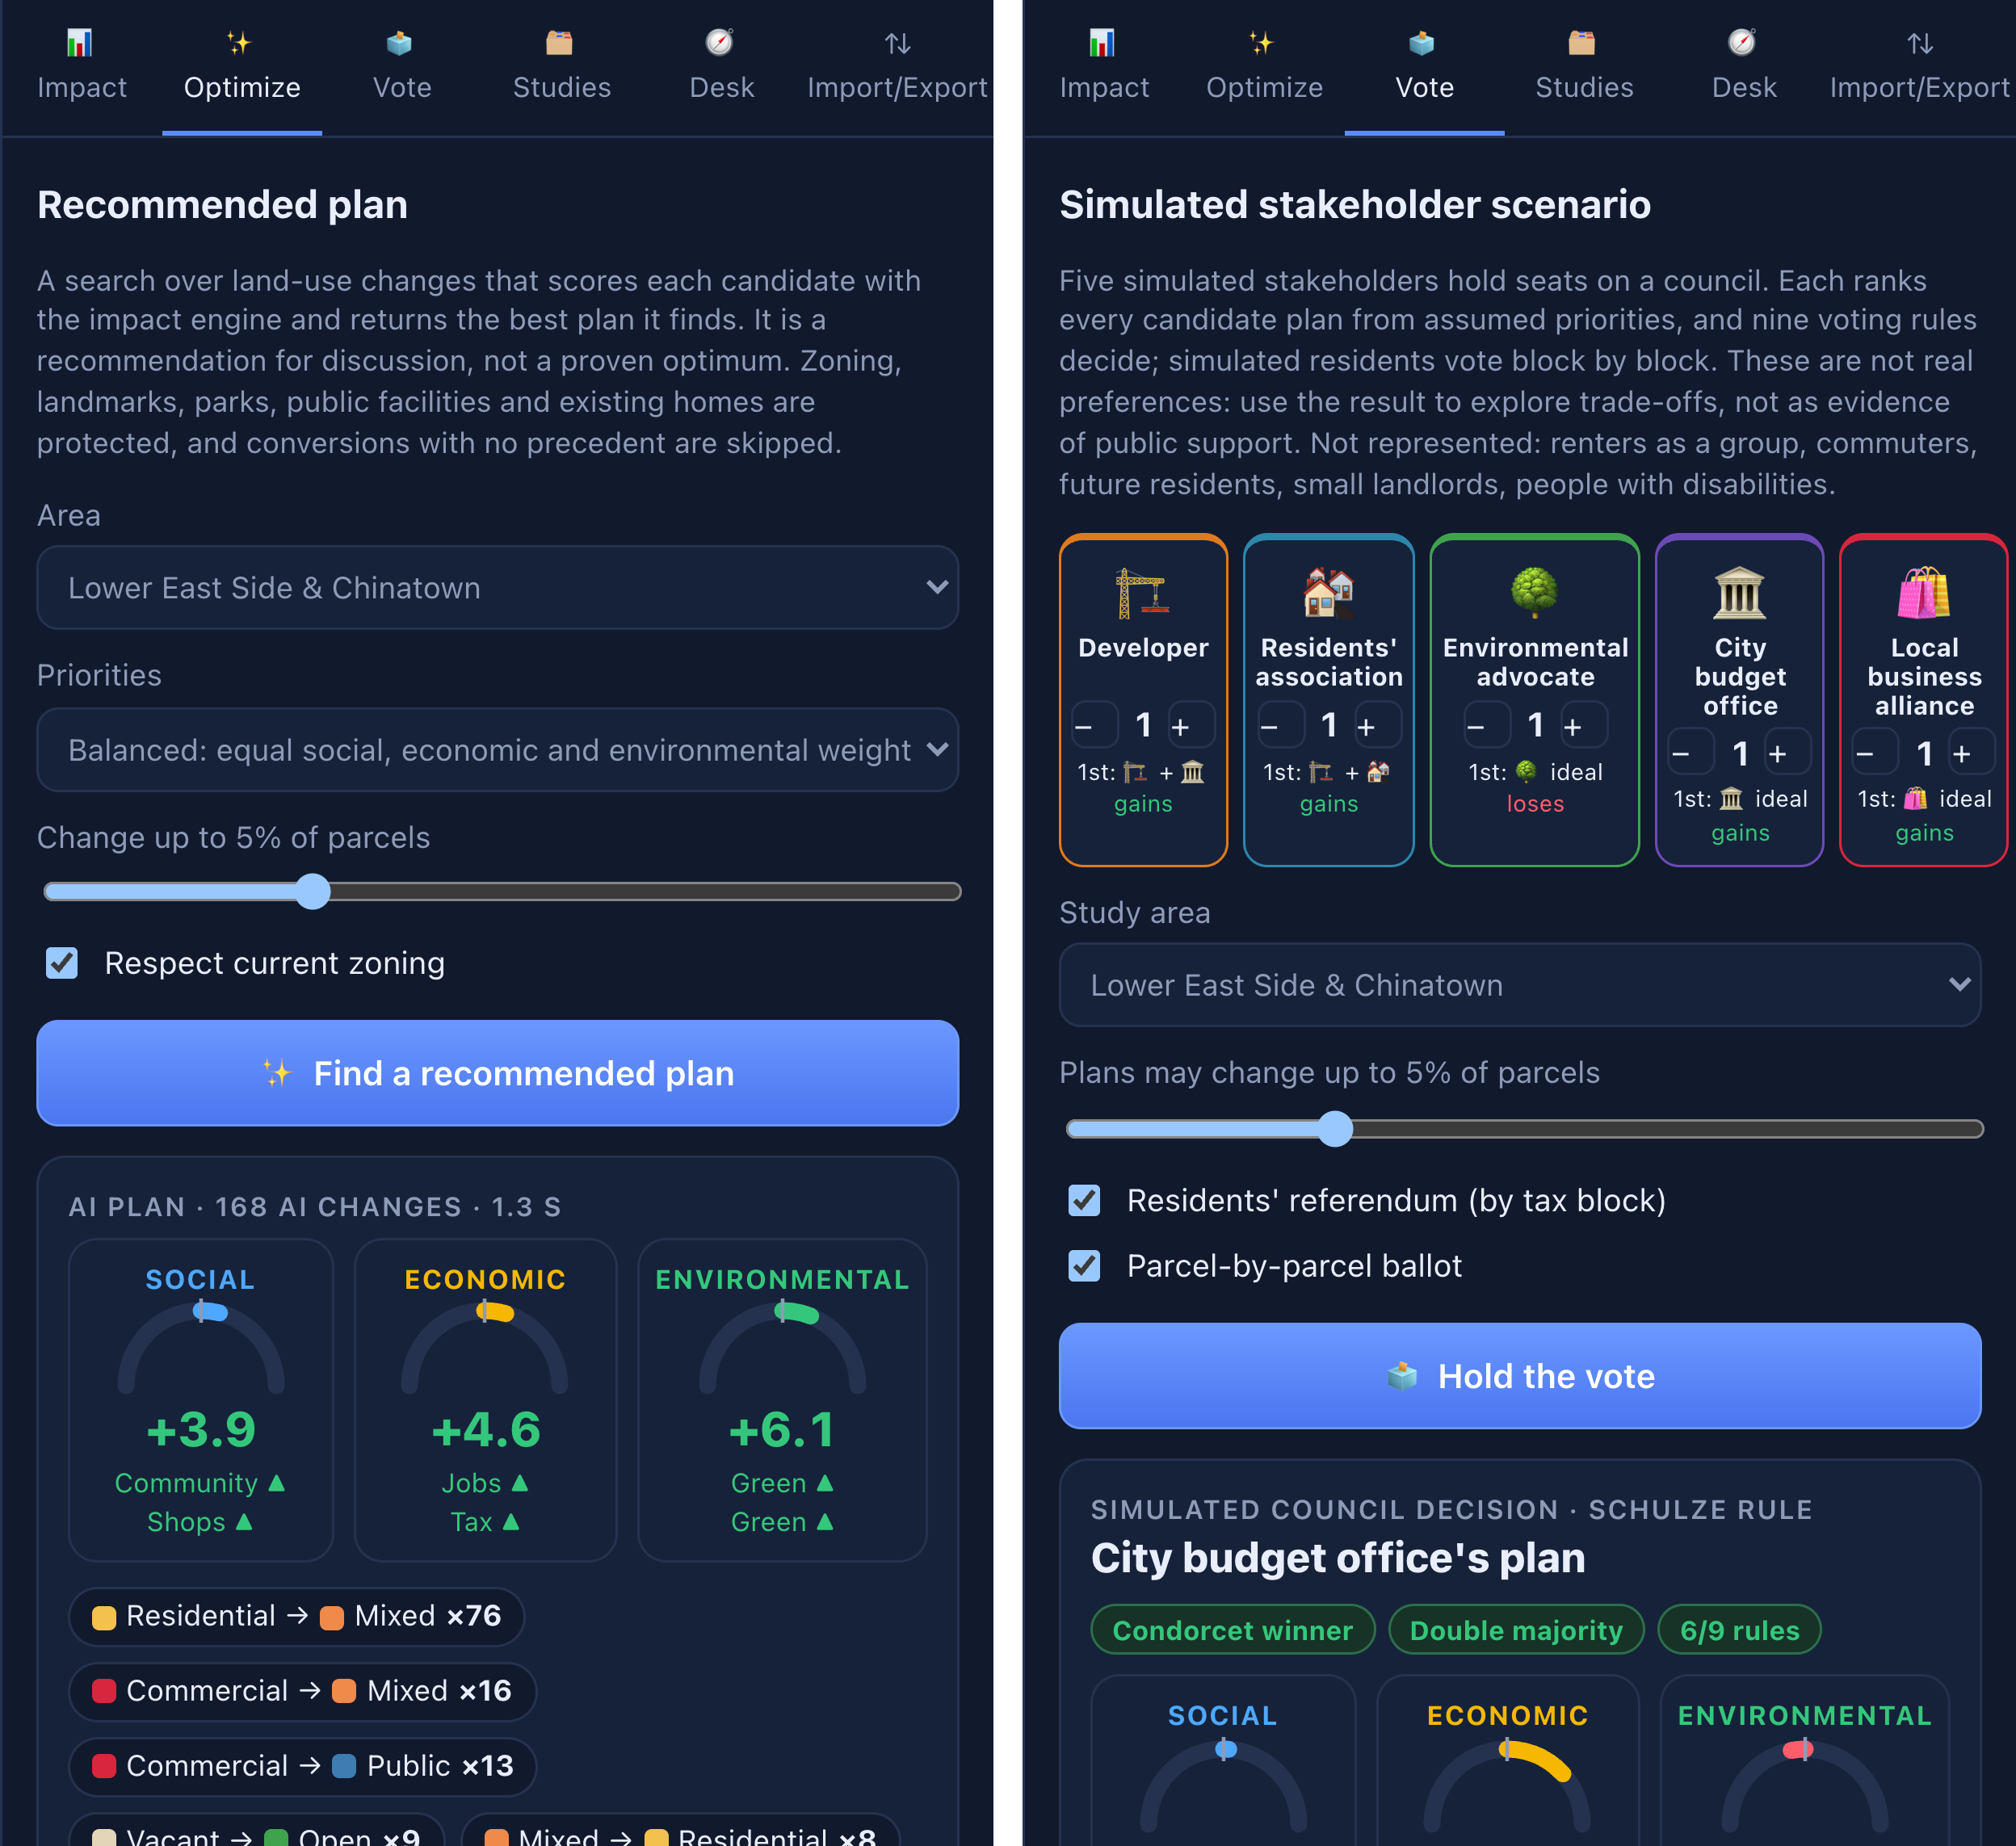
\includegraphics[width=0.8\linewidth]{ui_optimizer_vote.png}
\caption{Optimizer and decision module for one Manhattan district. Left: the recommended plan, its change in each
pillar and its conversions. Right: the simulated council's decision under Schulze's rule, whether the winner is a
Condorcet winner with a double majority, and how many of the nine rules it wins.}
\label{fig:optvote}
\end{figure}

\paragraph{Interface.} Planners can edit parcels by click, box, lasso or search, or upload plans as tables or GIS
files, which are reviewed before they are applied. Studies are stored with a hash-chained audit log. Exports include a
staff-report draft, CSV and GeoJSON files, and the provenance of every coefficient. A phone version presents the engine
as a game. Any city or district exports to ArcGIS Urban: space-use, zoning and land-use types, boundaries, and parcels
with a PlanArena scenario.

\section{Validation design}\label{sec:validation}

The claims rest on four kinds of evidence (Table~\ref{tab:design}): \emph{empirical predictive tests}, in which a
prediction made with earlier information is compared with a later outcome on observations not used to build or select
the model; \emph{accounting checks}, in which the twin reproduces records it was built from; \emph{algorithmic
verification} of the searches against exhaustive enumeration; and \emph{illustrative simulation} for the decision
module, which has no observed counterpart.
\begin{itemize}
\item \textbf{Time.} Predictions are trained on one period and tested on a later one; uncertainty comes from
resampling spatial tiles \citep{kunsch1989}, never from random splits \citep{roberts2017}. The cross-city test uses
seven cities with parcel histories (Appendix Table~\ref{tab:panels}).
\item \textbf{Development} is defined as each source records it: a new building or large floor-area increase (Los
Angeles, Dallas, New York), a new building (Milwaukee), a change of use class between land-use inventories (Phoenix,
San Diego), or a new-construction permit (Chicago). A building already on the starting record is never counted as new.
\item \textbf{Blocks.} Four feature blocks are added in turn: existing conditions (E), context within 400 m (C),
zoning (Z) and plan (P).
\item \textbf{Leakage control.} Every feature family is dated against the decision year (Supplement S2). Where a current
zoning or plan layer has dated changes, a conservative variant drops lots whose zoning or plan dates from the window's
start or later; lots that merge or split are followed by their representative point.
\end{itemize}

\begin{table}[t]
\centering
\scriptsize
\setlength{\tabcolsep}{4pt}
\caption{Evaluation design: each component, its question, data and type of evidence.}
\label{tab:design}
\begin{tabular}{lp{5.0cm}p{4.0cm}ll}
\toprule
Component & Question & Data & Evidence & Section \\
\midrule
Existing conditions & Does the twin reproduce what is there? & LL84 energy, LODES jobs, recorded homes & accounting & \ref{sec:r-existing} \\
Planning calculations & Does it reproduce a review's projection from the review's own inputs? & FEIS site tables (two rezonings) & accounting & \ref{sec:r-existing} \\
Effects of change & Given an observed change, does it predict the effect? & MapPLUTO 2015 vs 2025, held-out folds & empirical & \ref{sec:r-change} \\
Likelihood & Does it rank lots that redevelop, and how many, forward in time? & Rolling origins 2016--2025 & empirical & \ref{sec:r-likely} \\
Official layers & What do zoning and plans add, in other cities? & Seven city panels & empirical & \ref{sec:r-layers} \\
Housing projections & Are projected homes close to what was built? & Four cities; three rezonings & empirical & \ref{sec:r-homes} \\
Optimizer & How close is the best plan found to the best plan? & Exhaustive search; 12 districts & algorithmic & \ref{sec:r-opt} \\
Pareto explorer & Does NSGA-III find the trade-off front? & Exhaustive enumeration of blocks & algorithmic & \ref{sec:r-opt} \\
Realism & Are recommended changes plausible? & 2020 plans vs 2025 outcomes & empirical & \ref{sec:r-opt} \\
Decision module & How does the choice depend on rule, seats and candidates? & Assumed utilities & illustrative & \ref{sec:r-dec} \\
\bottomrule
\end{tabular}
\end{table}

\section{Results}\label{sec:results}

\subsection{Existing conditions and planning calculations}\label{sec:r-existing}

The twin reproduces Manhattan's existing conditions
(accounting checks).
\begin{itemize}
\item \textbf{Emissions.} Modelled emissions match 6{,}234 benchmarked buildings in a year not used for fitting
(log--log $r = 0.807$, median error 31\%, total 1.04 times metered).
\item \textbf{Jobs} correlate with LEHD counts at tract level ($r = 0.843$) and block level ($r =
0.727$).
\item \textbf{Homes.} Given observed use and floor area, homes on 295 lots developed in 2015--2025 total
1.04 times the recorded count ($r = 0.903$).
\item \textbf{Environmental reviews.} Given two rezoning reviews' own sites, floor area and uses, PlanArena reproduces
their projected homes at 0.86 and 1.00 times the review figures.
\end{itemize}

\subsection{Effects of observed change}\label{sec:r-change}

3{,}350 Manhattan lots changed use or floor area substantially between 2015 and 2025. Each was given its 2015
state and its observed new use and floor area, with coefficients from 2015 data. The test is conditional: it checks
the engine given what was built, not whether the change would happen. The delta form, the unit-size rule and a scale
factor were chosen on 1{,}314 lots in two of five spatial folds; results are for the other 2{,}036
(Table~\ref{tab:change}; Supplement S4).
\begin{itemize}
\item \textbf{Homes}: predicted change correlates with recorded change at $r = 0.79$, against
0.68 for gradient-boosted regression and 0.39 for the mean change of the same transition,
both fitted on the selection lots with the same information. The mean absolute error is 12.5 homes per lot,
against 16.5 for predicting no change.
\item \textbf{Value}: $r = 0.74$, against 0.57, but the direction of the change (relative
to the district trend) is right for only 60\% of lots, against 88\% for homes;
\textbf{emissions} of 115 benchmarked buildings: $r = 0.60$, against 0.36.
\item \textbf{Bias.} The engine overstates total homes added 1.47-fold (the regression baseline
1.24-fold). A scale factor fitted on the selection lots brings this to 1.35.
Conversions to mixed use account for 70\% of the excess; commercial-to-mixed conversions alone overstate by
28 homes per lot.
\item \textbf{Jobs.} By census block, predicted job change does not correlate with the change in LEHD counts
($r = 0.05$): the engine has no skill for job change at this scale.
\end{itemize}
Access, mix, green cover and runoff have no after-change data, and the Studio marks them as not validated.

\begin{table}[t]
\centering
\scriptsize
\setlength{\tabcolsep}{3pt}
\caption{Effects of observed change on 2{,}036 held-out Manhattan lots, 2015--2025: given the 2015 state and the observed new use and floor area, predicted against recorded change (Pearson $r$; mean absolute error and mean bias in homes per lot; predicted over observed total).}
\label{tab:change}
\begin{tabular}{lrrrrrrrr}
\toprule
Method & Homes $r$ & MAE & Bias & Total & Value $r$ & Total & Emis.\ $r$ & Total \\
\midrule
PlanArena (deployed form) & 0.79 & 12.5 & 5.6 & 1.47 & 0.74 & 0.70 & 0.60 & 1.24 \\
PlanArena (form chosen on selection lots) & 0.79 & 12.7 & 6.1 & 1.51 & 0.74 & 0.70 & 0.60 & 1.24 \\
\quad $\times$ selection-lot scale & 0.79 & 11.8 & 4.2 & 1.35 & 0.74 & 1.09 & 0.60 & 1.06 \\
Gradient-boosted regression & 0.68 & 15.4 & 2.9 & 1.24 & 0.57 & 1.19 & 0.36 & 1.10 \\
Mean change of the same transition & 0.39 & 22.3 & 1.5 & 1.12 & 0.10 & 1.07 & 0.26 & 2.26 \\
\bottomrule
\end{tabular}
\par\smallskip
\begin{minipage}{0.95\linewidth}\footnotesize Selection lots (1{,}314, two of five spatial folds) chose the form and fitted the baselines and the scale. Predicting no change gives a homes MAE of 16.5. Emissions: 115 benchmarked buildings.\end{minipage}
\end{table}

\subsection{Likelihood of redevelopment}\label{sec:r-likely}

Trained on 2015--2020 outcomes and tested on 2020--2025, the redevelopment model reaches AUC 0.855, against
0.802 for the best simple baseline and 0.833 for a graph neural network, with 26\%
redeveloped among its top 1\% of lots against a base rate of 1.23\%. Across 15 rolling origins
(2016--2025; horizons of one, three and five years), its out-of-time AUC is 0.851--0.902, above the
best baseline at every origin.

\paragraph{Calibration} (Supplement S5). The model ranks lots better than it predicts how many redevelop.
\begin{itemize}
\item \textbf{Totals shift with the cycle.} Observed over predicted redevelopments ranged from 0.07 to
1.70 across origins, and in the seven cities' test windows from 0.42 to 1.60.
\item \textbf{Spread.} Calibration slopes were 0.59--0.95: the probabilities are too spread
out.
\item \textbf{Skill.} Against a constant forecast of the training-period rate, Brier skill was $-$0.97 to
0.15, negative at three of 15 origins.
\item \textbf{Recalibration} on out-of-fold training probabilities corrects the spread (slopes
0.74--1.05) but not the totals, which still range 0.06--1.31
in Manhattan and 0.41--1.24 in the cities: the rate of development changes between
windows in ways a model trained on earlier windows does not anticipate.
\end{itemize}
The probabilities are used to rank sites and to weight projections whose totals are compared with observed rates, not
as forecasts of how many lots will redevelop.

\subsection{What zoning and plans add, across seven cities}\label{sec:r-layers}

Existing conditions alone rank developed lots with out-of-time AUC 0.824--0.911 in six cities, and
0.571 in San Diego, whose one-year window recorded few changes (Appendix Table~\ref{tab:auc}). Adding blocks:
\begin{itemize}
\item \textbf{Context} adds the most: +0.021 to +0.116, significant in five cities
(Table~\ref{tab:gains}, Figure~\ref{fig:gains}). Phoenix is the exception: its land-use series starts in 2022, so
recent change is unknown in its training window.
\item \textbf{Zoning} carries its own signal. Without context, it raises AUC significantly in five of seven cities, and
developed lots were 2.1--9.5 times as likely as others to have a zoning class outside
their existing use group.
\item \textbf{Overlap.} Most of that signal is shared with existing conditions and context: developed lots were also
3.5--19 times as likely to be vacant. Over context, zoning adds a significant gain in
five of seven cities and the plan in three of four, at most +0.021 outside Phoenix.
\item \textbf{Phoenix.} Zoning adds +0.049 and the plan +0.054, and 45\% of developed lots were
vacant.
\item \textbf{Conservative variant.} The plan gain in San Diego and the zoning gain in Chicago do not survive it: those gains came from lots rezoned or
re-planned during the study. Dallas's zoning and plan are undated current layers (the plan was adopted after the
window's start), so its zoning and plan results may contain post-decision information.
\end{itemize}

The layers matter more for what developing lots become (Table~\ref{tab:dest}).
\begin{itemize}
\item \textbf{Zoning class.} In all six cities with a destination, it names the new class correctly more often
than the existing use does, by 12--64 percentage points. In Phoenix and San Diego, development
is a change of class by definition, so the existing use is never right at class level.
\item \textbf{Plan class.} In Dallas it is right for 80\% of developed lots, against 61\%
for zoning.
\item \textbf{Transfer.} Models fitted on other cities predict worse than the city's own in four of five cities
(Appendix Table~\ref{tab:transfer}).
\end{itemize}

\begin{table}[t]
\centering
\scriptsize
\setlength{\tabcolsep}{2.5pt}
\caption{Gain in out-of-time AUC from adding a block, with 95\% bootstrap intervals over 2 km tiles. Bold: the interval excludes zero.}
\label{tab:gains}
\begin{tabular}{llllll}
\toprule
City & C over E & Z over E+C & P over E+C & Z, conservative & P, conservative \\
\midrule
Los Angeles & \textbf{+0.027 [0.020, 0.034]} & \textbf{+0.005 [0.001, 0.008]} & +0.002 [$-$0.002, 0.006] &  &  \\
Dallas & \textbf{+0.021 [0.016, 0.026]} & \textbf{+0.003 [0.002, 0.005]} & \textbf{+0.002 [0.001, 0.003]} &  &  \\
New York & \textbf{+0.023 [0.018, 0.029]} & \textbf{+0.004 [0.003, 0.007]} & -- &  &  \\
Milwaukee & $-$0.015 [$-$0.079, 0.048] & +0.029 [$-$0.031, 0.075] & -- &  &  \\
Phoenix & $-$0.066 [$-$0.139, 0.001] & \textbf{+0.049 [0.009, 0.091]} & \textbf{+0.054 [0.005, 0.100]} & \textbf{+0.055 [0.017, 0.088]} & \textbf{+0.041 [0.004, 0.073]} \\
San Diego & \textbf{+0.116 [0.053, 0.170]} & $-$0.003 [$-$0.022, 0.018] & \textbf{+0.021 [0.003, 0.039]} & $-$0.009 [$-$0.029, 0.015] & $-$0.011 [$-$0.033, 0.007] \\
Chicago & \textbf{+0.063 [0.049, 0.078]} & \textbf{+0.004 [0.001, 0.007]} & -- & $-$0.001 [$-$0.005, 0.003] & -- \\
\bottomrule
\end{tabular}
\par\smallskip
\begin{minipage}{0.95\linewidth}\footnotesize Conservative: in each window, lots whose zoning or plan dates from the window's start or later are left out; possible where a current layer records those dates (Phoenix, San Diego, Chicago). Dallas's current layers carry no dates, so its zoning and plan gains may include post-decision information.\end{minipage}
\end{table}

\begin{figure}[t]
\centering
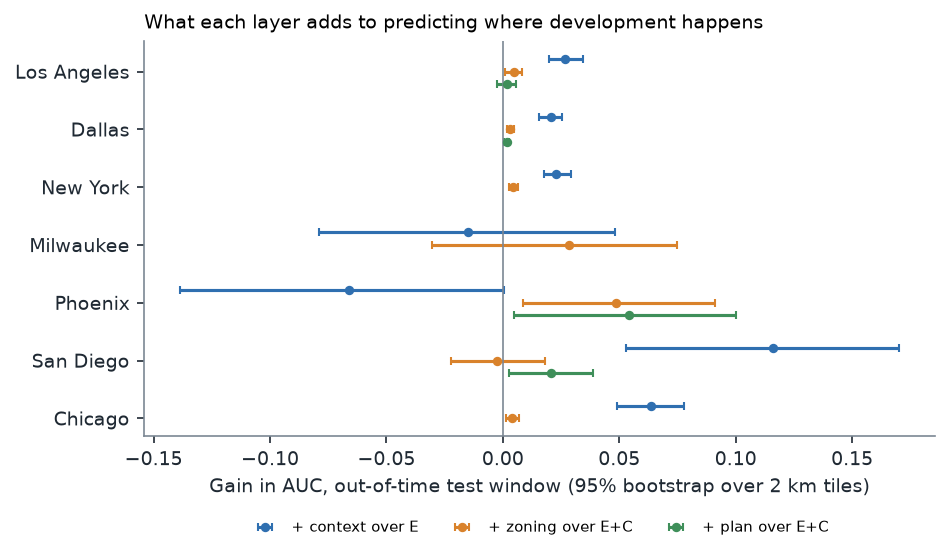
\includegraphics[width=0.66\linewidth]{integration_layers.png}
\caption{Gain in out-of-time AUC from each block, with 95\% tile-bootstrap intervals.}
\label{fig:gains}
\end{figure}

\begin{table}[t]
\centering
\scriptsize
\setlength{\tabcolsep}{4pt}
\caption{What developed lots became: share named correctly, as one of 16 classes / one of nine groups.}
\label{tab:dest}
\begin{tabular}{lrllll}
\toprule
City & Developed & No change & Zoning class & Plan class & Model (blocks) \\
\midrule
Los Angeles & 1{,}877 & 57\% / 79\% & 70\% / 87\% & 70\% / 87\% & 75\% / 89\% (E+C+Z+P) \\
Dallas & 3{,}886 & 37\% / 40\% & 61\% / 65\% & 80\% / 90\% & 86\% / 96\% (E+C+Z+P) \\
New York & 4{,}002 & 24\% / 37\% & 49\% / 65\% & -- & 54\% / 70\% (E+Z) \\
Milwaukee & 78 & 18\% / 18\% & 37\% / 77\% & -- & 63\% / 76\% (E+Z) \\
Phoenix & 1{,}835 & 0\% / 35\% & 64\% / 74\% & 47\% / 62\% & 75\% / 81\% (E+C+Z+P) \\
San Diego & 202 & 0\% / 52\% & 14\% / 74\% & 27\% / 70\% & 64\% / 75\% (E+C+Z+P) \\
\bottomrule
\end{tabular}
\par\smallskip
\begin{minipage}{0.95\linewidth}\footnotesize In Phoenix and San Diego development is a change of class (to another group, or to more homes), so ``no change'' is never right at class level there. Models are cross-fitted over 2 km tiles among the developed lots. Chicago's permits do not record the new use.\end{minipage}
\end{table}

\subsection{Housing projections}\label{sec:r-homes}

Projections and observations differ in kind: build-out is an end state, while the observed count is the gross number
of homes added in a two- or four-year window (Table~\ref{tab:homes}).
\begin{itemize}
\item \textbf{Ranking districts.} A five-year trend ranks districts better than build-out and likelihood $\times$
build-out in all four cities: Spearman 0.51 to 0.81, against $-$0.37 to 0.55.
Likelihood $\times$ empirical yield (below) reaches $-$0.28 to 0.83, as well as the trend or better
in three of four.
\item \textbf{Build-out.} A proxy of zoning and plan build-out (each lot at the density that lots of its zoned or
planned class reach today, not legal capacity) exceeds the homes added in the window 76- to 193-fold.
\item \textbf{Totals.} Likelihood weighting brings totals to 0.80--2.60 times the observed. Using the homes
that developing lots of the same class and size added in the training window instead of build-out gives
0.12--0.45: it ranks districts well but underestimates how many homes are built.
\item \textbf{Manhattan rezonings} (Table~\ref{tab:replay}, Figure~\ref{fig:replay}). Capacity projected
8{,}423 homes on development sites, or 5{,}207 pro-rated to 2025; 561 were built.
Probability $\times$ capacity gave 607, but the close total comes from errors that cancel: 0.84 and
0.87 times the observed in East Harlem and Inwood, and 44 times in SoHo/NoHo, where
3 homes were built. Soft sites redeveloped in the training years added 38\%--102\% of their capacity
homes on average; scaling by that share gives 352 in total and a larger summed error across the three
(471 homes, against 212), so the empirical yield did not improve these projections. The observed
count lies within the 95\% range of probability $\times$ capacity in two of three rezonings; the ranges are conditional
on the model's probabilities and omit model error.
\end{itemize}

\begin{table}[t]
\centering
\scriptsize
\setlength{\tabcolsep}{3pt}
\caption{Homes added in the test window: projection over observed total (Spearman correlation across districts).}
\label{tab:homes}
\begin{tabular}{lrllllll}
\toprule
City & Observed & Zoning build-out & Plan build-out & Likely $\times$ zoning & Likely $\times$ plan & Likely $\times$ yield & Five-year trend \\
\midrule
Los Angeles & 22{,}853 & 193$\times$ (0.10) & 189$\times$ (0.24) & 0.80$\times$ (0.51) & 0.81$\times$ (0.54) & 0.33$\times$ (0.79) & 0.59$\times$ (0.70) \\
Dallas & 10{,}926 & 141$\times$ (0.00) & 127$\times$ (0.34) & 2.60$\times$ ($-$0.05) & 1.59$\times$ (0.33) & 0.45$\times$ (0.73) & 1.25$\times$ (0.72) \\
New York & 116{,}776 & 76$\times$ (0.34) & -- & 0.96$\times$ (0.55) & -- & 0.37$\times$ (0.83) & 0.47$\times$ (0.81) \\
Milwaukee & 3{,}798 & 115$\times$ ($-$0.23) & -- & 0.97$\times$ ($-$0.37) & -- & 0.12$\times$ ($-$0.28) & 0.32$\times$ (0.51) \\
\bottomrule
\end{tabular}
\par\smallskip
\begin{minipage}{0.95\linewidth}\footnotesize Observed: gross homes added in the window. Build-out (a proxy, not legal capacity): every lot at the homes per acre that the 90th percentile of lots of its zoned (or planned) class reach in the city today. Likely: the build-out increment times the out-of-time probability of development (blocks E+C+Z+P where available). Yield: the probability times the mean homes added by developing lots of the same class and lot size in the training window. Trend: homes completed in the five years before the window, scaled to its length.\end{minipage}
\end{table}

\begin{table}[t]
\centering
\footnotesize
\setlength{\tabcolsep}{3pt}
\caption{Three Manhattan rezonings: homes on development sites by 2025, observed and projected.}
\label{tab:replay}
\begin{tabular}{lrrrrll}
\toprule
Rezoning (adopted) & Sites & Built & Capacity & Pro-rated & Prob.\ $\times$ capacity (95\%) & Prob.\ $\times$ yield (95\%) \\
\midrule
East Harlem (2017) & 127 & 288 & 4{,}117 & 3{,}294 & 241 (82--497) & 91 (0--444) \\
Inwood (2018) & 47 & 270 & 2{,}859 & 1{,}334 & 234 (0--677) & 127 (0--1{,}033) \\
SoHo/NoHo (2021) & 77 & 3 & 1{,}447 & 579 & 132 (8--296) & 134 (0--801) \\
\textit{All three} &  & 561 & 8{,}423 & 5{,}207 & 607 & 352 \\
\textit{Sum of absolute errors} &  &  & 7{,}862 & 4{,}646 & 212 & 471 \\
\bottomrule
\end{tabular}
\par\smallskip
\begin{minipage}{0.95\linewidth}\footnotesize Capacity is full build-out by the review's build year; pro-rated scales it linearly to 2025. The probability comes from a redevelopment model trained only on outcomes known by the adoption year; yield is the mean share of capacity homes that soft sites redeveloped in those training years added. Ranges are conditional on the probabilities (Supplement S5).\end{minipage}
\end{table}

\begin{figure}[t]
\centering
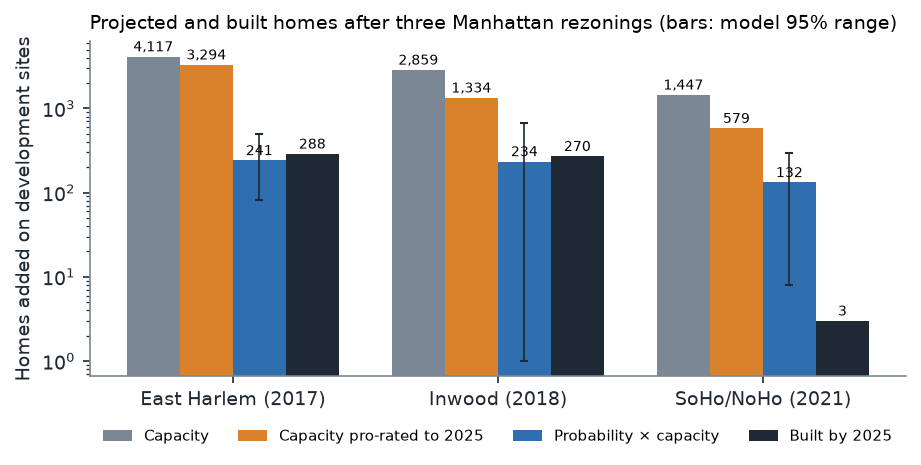
\includegraphics[width=0.66\linewidth]{integration_replay.png}
\caption{Homes on development sites after three Manhattan rezonings: capacity, pro-rated capacity,
probability $\times$ capacity (with its 95\% range, conditional on the probabilities) and built by 2025 (log scale).}
\label{fig:replay}
\end{figure}

\subsection{Optimizer and plausibility}\label{sec:r-opt}

\paragraph{Optimality} (algorithmic verification). In 20 small areas (one tax block each) every plan with up
to two changes was enumerated, and 15 had a plan better than no change. First-order search found the optimum
in 14 of 15 of these, and with exact re-scoring in all 15 (median 0.51 s). At district
scale no method guarantees an optimum, so methods are compared with the best plan any of them found
(Table~\ref{tab:opt}): exact greedy search found it in all 12 districts but took a median 36.15 s;
first-order search with re-scoring reached a median 95.7\% of it in 1.88 s, the speed used in
the Studio.

\paragraph{Trade-off front.} On ten tax blocks with 24{,}576--327{,}680 possible plans each, the NSGA-III
explorer's front covered a median 100.0\% (minimum 98.6\%) of the hypervolume of the exhaustive
front, against 96.4\% for random search with as many evaluations; on ten smaller blocks scored
exactly, it recovered the exact front. The test exposed terms missing from the first-order model, since added
(Supplement S6).

\paragraph{Plausibility} (Table~\ref{tab:realism}). Plans were recommended on the 2020 snapshot and compared with 2025,
with the same number of recommended parcels in each setting and one objective.
\begin{itemize}
\item \textbf{Precedent.} Without realism layers, 17\% of recommended changes had no precedent.
\item \textbf{Redevelopment.} Recommended parcels were redeveloped by 2025 at 11\% without realism layers,
15\% with the precedent filter and 21\% with the likelihood layer, against 1.2\% of all lots
and 5.0\% of the likeliest fifth.
\item \textbf{Redevelopment is not implementation.} None of the recommended parcels became the recommended use.
\item \textbf{The cost.} The objective fell by 3\% with the precedent filter and 48\% with the
likelihood layer: the filter removes implausible conversions at little cost, while restricting candidates to likely
sites trades much of the objective for plausibility.
\end{itemize}

\begin{table}[t]
\centering
\small
\setlength{\tabcolsep}{4pt}
\caption{Optimizer at district scale (12 Manhattan districts, up to ten changes): share of the best plan any tested method found (not a proven optimum).}
\label{tab:opt}
\begin{tabular}{lrrr}
\toprule
Search & Median share of best & Districts best & Median seconds \\
\midrule
surrogate top moves & 91.0\% & 0 & 0.02 \\
first order & 94.1\% & 0 & 0.25 \\
first order plus exact polish & 95.7\% & 1 & 1.88 \\
greedy exact & 100.0\% & 12 & 36.15 \\
simulated annealing & 93.6\% & 0 & 10.65 \\
random restarts 50 & 65.5\% & 0 & 1.31 \\
\bottomrule
\end{tabular}
\end{table}

\begin{table}[t]
\centering
\scriptsize
\setlength{\tabcolsep}{4pt}
\caption{Realism layers at equal counts: plans recommended on the 2020 snapshot of every Manhattan district, and what happened by 2025.}
\label{tab:realism}
\begin{tabular}{lrrrrrr}
\toprule
Optimizer setting & Parcels & No precedent & Redeveloped & Eligible redev. & Into rec.\ use & Objective \\
\midrule
no realism layer & 116 & 16.4\% & 11.2\% & 1.5\% & 0.0\% & 83.7 \\
precedent filter (default) & 117 & 0.0\% & 15.4\% & 1.5\% & 0.0\% & 81.3 \\
precedent filter + likelihood layer & 118 & 0.0\% & 21.2\% & 5.0\% & 0.0\% & 43.4 \\
\bottomrule
\end{tabular}
\par\smallskip
\begin{minipage}{0.95\linewidth}\footnotesize In each district every setting recommends the smallest number any setting recommended there. Eligible redev.: share of the setting's eligible parcels redeveloped (the rate of a random choice). Objective: the sum over districts of the overall score minus the conversion penalty. At the full budget the settings recommended 539, 543, 118 parcels.\end{minipage}
\end{table}

\subsection{Decision rules (illustrative)}\label{sec:r-dec}

The decision module has no observed counterpart: its outputs follow from assumed utilities, one seat per agent and the
generated candidates. In the simulated scenario for 12 Manhattan districts:
\begin{itemize}
\item the nine rules never all agree, and a Condorcet winner exists in seven;
\item the residents' referendum picks the council's plan in one district, and the council's winner
is never the Nash bargaining solution;
\item one insincere ballot could change the Schulze result in eight districts;
\item the winner survives a median 68\% of joint perturbations of coefficients and seats, and 58\%
of redrawn agent weights;
\item the candidates matter: the nine rules pick a median of four distinct winners on the generated
ballot, three on the agents' ideal plans alone and two on random feasible plans;
\item with resident weights drawn independently for each block, the residents' winner is unchanged in a median
100\% of draws.
\end{itemize}
These describe the simulated scenario, not public opinion. They make explicit what a hearing leaves implicit: resident
and environmental interests are inputs to the decision, and a recommendation should be reported with its rule, its
candidates and how it changes under others.

\section{Discussion}\label{sec:discussion}

\paragraph{What a planner gets.} For any proposed change, PlanArena shows:
\begin{itemize}
\item its effects on 11 indicators, with ranges;
\item whether zoning and the plan allow it, and how likely it is;
\item what the optimizer would recommend instead;
\item how the choice depends on the decision rule.
\end{itemize}
Each output has a stated test and type of evidence (Table~\ref{tab:design}), and untested indicators are
labelled. For one system, this narrows the gap between claimed and demonstrated contributions of PSS and urban twins
\citep{vonk2005,azadi2025,kruse2026}.

\paragraph{Design guidance.}
\begin{enumerate}
\item \textbf{Use each layer for the question it answers.} Once existing conditions and context were known, zoning and
plans added little to ranking \emph{where} development happened in these windows. They helped name \emph{what} it
became and bound \emph{how much} a site can hold. This is consistent with rezoning following opportunity \citep{gabbe2018},
upzoning's varying short-run effects \citep{freemark2020,dong2024,greenaway2023} and partial plan implementation
\citep{laurian2004,berke2006}.
\item \textbf{Report a trend first, and likelihood-weighted projections beside capacity.} Capacity overstates
near-term housing by orders of magnitude. A trend ranked districts better than build-out-based projections in all four cities, and likelihood $\times$ yield as well as the trend in three of four. Close totals can hide large errors by area.
\item \textbf{Constrain optimization by plausibility and show the cost.} Realism layers change recommendations and
lower the objective; recommended sites that redevelop rarely become the recommended use.
\item \textbf{Report decisions with their rule.} No rule agreed with all the others in any district of the simulated scenario.
\end{enumerate}

\paragraph{Limitations.}
\begin{itemize}
\item \textbf{Impacts} are evaluated only in Manhattan and only given what was built; in the other nine cities they
are unvalidated estimates from national or regional coefficients.
\item \textbf{Indicators without skill or test.} Job change by block was tested and showed no skill; access, mix,
green cover and runoff after a change have no observed test.
\item \textbf{Calibration.} Redevelopment probabilities shift with the market cycle, so expected totals need checking
against recent rates.
\item \textbf{The cross-city test} uses short windows (one or two years) and city-specific outcome definitions, and
Dallas's undated layers may include post-decision information.
\item \textbf{Representation.} Zoning is reduced to use permissions and maximum floor-area ratios (no height, bulk,
parking or bonus rules), access to straight-line distance, and uncertainty to sensitivity ranges, which are not
prediction intervals.
\item \textbf{Distribution.} Indicators are averages over a scope. Who gains and who loses within it (by income,
tenure or race), displacement and the effects on future residents are not measured.
\item \textbf{Decisions.} The optimizer is heuristic, and the votes rest on assumed utilities and one seat per
interest, not on elicited preferences or representation.
\item \textbf{Not studied.} Usability with planners is not evaluated, and causal effects of zoning or plans are not
estimated.
\end{itemize}

\section{Conclusion}

Land-use and location decisions have multidimensional, spatially interacting and uncertain effects, yet they are
decided at hearings where those effects are summarised in a few indicators and residents do not vote. PlanArena, a
land-use optimizer, measures the effects of any parcel-level change on social, economic and environmental
indicators, with what is permitted, planned, likely and recommended, and turns stakeholder interests into votes. It runs on official data for ten large US cities
at interactive speed, and each component has a stated test, empirical where data allow. The tests also shape the
design:
\begin{itemize}
\item once existing conditions and context are known, regulatory layers mainly inform what development becomes and
how much it could hold;
\item a five-year trend ranked districts better than build-out projections, and likelihood-weighted totals were far
closer to what was built than capacity, partly through errors that cancel;
\item recommendations change when they must be plausible, at a measured cost, and the chosen plan changes with the
rule and the candidates.
\end{itemize}
Code, data manifest and results are released with the paper, so the system and its tests extend to other cities.

\paragraph{Data and code availability.} The code, the result files behind every number, the figures and a manifest
of every input (URL, retrieval date, SHA-256) are in the PlanArena repository, release \texttt{v1.1-review}
[public repository URL and archived DOI to be added by the author]. The technical supplement specifies every model and
test. \texttt{make reproduce} rebuilds data
and results from public sources, and \texttt{planarena/tools/screenshots.py} regenerates the Studio figures. Each
city's ingestion report documents coverage, crosswalks and estimated fields. Owner and mailing fields in assessor
records were never requested or read. No human participants were involved.

\paragraph{Declaration of AI assistance.} [To be confirmed by the author.] The author used Claude (Anthropic), through
Claude Code, to write and test code, run analyses, and draft the text and the supplement. The author designed the
study and the system, reviewed the code, results and text, read the cited sources and takes responsibility for the
content. Every reference was checked against the record its DOI or ISBN resolves to. No AI system generated data or
results; every number is computed by the released code.

\appendix
\section{Digitising plans published as PDF maps}\label{app:digitise}

Philadelphia2035's land-use recommendations exist only as ``Proposed Land Use'' maps in 17 district plans
covering 18 districts. Each lot is a filled vector shape. The maps are converted in six steps:
\begin{enumerate}
\item \textbf{Legend.} Swatch colours and labels are read.
\item \textbf{Colour matching.} Map colours are matched one to one to legend colours by CIELAB $\Delta E$ with a
Hungarian assignment, refusing pairs with $\Delta E > 45$.
\item \textbf{Visibility.} Only shapes the rendered page shows are kept, since maps are often clipped to the
district, and only the largest map frame on the spread.
\item \textbf{Registration.} A similarity transform is fitted. The rendered footprint is matched as an image to the
district's parcels and outline (FFT translation, Dice score), then refined by iterative closest point
\citep{reddy1996,besl1992,umeyama1991}.
\item \textbf{Classification.} Each parcel takes the category of the smallest shape containing its interior point.
\item \textbf{Checks.} A map is used only if the median parcel-to-shape distance is at most 10 ft, and its plan agrees
with existing use clearly more often than the same map shifted 300 ft.
\end{enumerate}
Results:
\begin{itemize}
\item \textbf{Coverage.} Maps from 15 of 17 plans passed, covering 16
districts and 83\% of parcels.
\item \textbf{Registration.} Median errors were 1.1--7.2 ft (median 3.2 ft).
\item \textbf{Shifted-map control.} The digitised plans agree with existing use on 60\%--90\%
of parcels, against 42\%--66\% for shifted maps.
\item \textbf{Independent reading.} Each parcel's category was also read from the colour of the rendered page around
its point, matched to the legend's rendered colours. On 451{,}691 parcels read both ways, the two readings agree
on 99.8\% (99.4\%--100.0\% by district). Both use the same registration, which the shifted-map
control checks. A random sample of 150 parcels, with page positions and map crops, is provided for a check
by eye against the PDFs.
\item \textbf{Failures.} The maps of South and West Park also draw neighbouring districts and failed registration.
\end{itemize}
Earlier work addresses scanned raster maps \citep{chiang2014,luft2021,milleville2022}; vector exports allow shapes to
be read directly.

\section{Additional results}
\FloatBarrier

\begin{table}[h!]
\centering
\scriptsize
\setlength{\tabcolsep}{4pt}
\caption{Test panels. Models are fitted on the training window and scored on the test window.}
\label{tab:panels}
\begin{tabular}{lllllrrr}
\toprule
City & Development & Source & Train & Test & Lots & Developed & Rate \\
\midrule
Los Angeles & new building or floor area +25\% & county assessor rolls & 2021--2023 & 2023--2025 & 667{,}844 & 2{,}215 & 0.33\% \\
Dallas & new building or floor area +25\% & appraisal district files & 2022--2024 & 2024--2026 & 291{,}841 & 3{,}892 & 1.33\% \\
New York & new building or floor area +25\% & MapPLUTO & 2021--2023 & 2023--2025 & 856{,}901 & 4{,}064 & 0.47\% \\
Milwaukee & new building & MPROP & 2021--2023 & 2023--2025 & 147{,}539 & 85 & 0.06\% \\
Phoenix & change of use group & MAG land-use inventory & 2022--2024 & 2024--2026 & 503{,}635 & 1{,}835 & 0.36\% \\
San Diego & change of use group & SANDAG land-use inventory & 2023--2024 & 2024--2025 & 272{,}281 & 202 & 0.07\% \\
Chicago & new-construction permit & building permits & 2021--2023 & 2023--2025 & 606{,}294 & 1{,}548 & 0.26\% \\
\bottomrule
\end{tabular}
\par\smallskip
\begin{minipage}{0.95\linewidth}\footnotesize Lots already under construction at the start of a window are left out. Floor area +25\% also requires +2,000 sq ft. Change of use group: the lot changes to a built use of another of the nine groups, or gains homes.\end{minipage}
\end{table}

\begin{table}[h!]
\centering
\small
\setlength{\tabcolsep}{4pt}
\caption{Where development happens: out-of-time AUC by block set. E existing conditions, C neighbourhood context, Z zoning, P adopted plan; -- where the city has no such layer.}
\label{tab:auc}
\begin{tabular}{lrrrrrl}
\toprule
City & E & E+C & E+C+Z & E+C+P & E+C+Z+P & Best set (any) \\
\midrule
Los Angeles & 0.863 & 0.889 & 0.894 & 0.891 & 0.894 & E+C+Z \\
Dallas & 0.897 & 0.917 & 0.921 & 0.919 & 0.922 & E+C+Z+P \\
New York & 0.892 & 0.914 & 0.919 & -- & -- & E+C+Z \\
Milwaukee & 0.911 & 0.896 & 0.924 & -- & -- & E+Z \\
Phoenix & 0.859 & 0.793 & 0.842 & 0.847 & 0.853 & E+Z+P \\
San Diego & 0.571 & 0.687 & 0.684 & 0.707 & 0.703 & E+C+P \\
Chicago & 0.824 & 0.888 & 0.891 & -- & -- & E+C+Z \\
\bottomrule
\end{tabular}
\par\smallskip
\begin{minipage}{0.95\linewidth}\footnotesize Best set: the highest AUC among all fitted combinations, including those without context.\end{minipage}
\end{table}

\begin{table}[h!]
\centering
\small
\setlength{\tabcolsep}{4pt}
\caption{Transfer: AUC of a model fitted on the other cities' training windows / the city's own model, on the city's test window.}
\label{tab:transfer}
\begin{tabular}{lllll}
\toprule
City & E & E+C & E+C+Z & E+C+Z+P \\
\midrule
Los Angeles & 0.726 / 0.863 & 0.822 / 0.889 & 0.827 / 0.894 & 0.828 / 0.894 \\
Dallas & 0.845 / 0.897 & 0.873 / 0.917 & 0.880 / 0.921 & 0.872 / 0.922 \\
New York & 0.824 / 0.892 & 0.871 / 0.914 & 0.874 / 0.919 & 0.865 / 0.919 \\
Milwaukee & 0.958 / 0.911 & 0.966 / 0.896 & 0.966 / 0.924 & 0.966 / 0.924 \\
Chicago & 0.736 / 0.824 & 0.805 / 0.888 & 0.800 / 0.891 & 0.814 / 0.891 \\
\bottomrule
\end{tabular}
\par\smallskip
\begin{minipage}{0.95\linewidth}\footnotesize Cities whose outcome is a building or a permit. A missing plan layer is coded as unknown.\end{minipage}
\end{table}

\begin{table}[h!]
\centering
\small
\setlength{\tabcolsep}{4pt}
\caption{Out-of-time average precision and precision among the top 1\% of lots.}
\label{tab:ap}
\begin{tabular}{lrrrlrr}
\toprule
City & Base rate & AP, E & AP, all & All blocks & Top 1\%, E & Top 1\%, all \\
\midrule
Los Angeles & 0.33\% & 0.132 & 0.143 & E+C+Z+P & 11.2\% & 12.7\% \\
Dallas & 1.33\% & 0.108 & 0.232 & E+C+Z+P & 11.8\% & 29.3\% \\
New York & 0.47\% & 0.073 & 0.122 & E+C+Z & 11.1\% & 15.1\% \\
Milwaukee & 0.06\% & 0.024 & 0.031 & E+C+Z & 2.3\% & 2.8\% \\
Phoenix & 0.36\% & 0.091 & 0.054 & E+C+Z+P & 9.7\% & 8.4\% \\
San Diego & 0.07\% & 0.002 & 0.002 & E+C+Z+P & 0.7\% & 0.6\% \\
Chicago & 0.26\% & 0.013 & 0.043 & E+C+Z & 2.4\% & 6.1\% \\
\bottomrule
\end{tabular}
\end{table}

\bibliographystyle{unsrtnat}
\bibliography{../docs/refs}

\end{document}
